\documentclass[tikz]{standalone}
\usepackage{pgfplots}
\pgfplotsset{compat=1.18}

\begin{document}

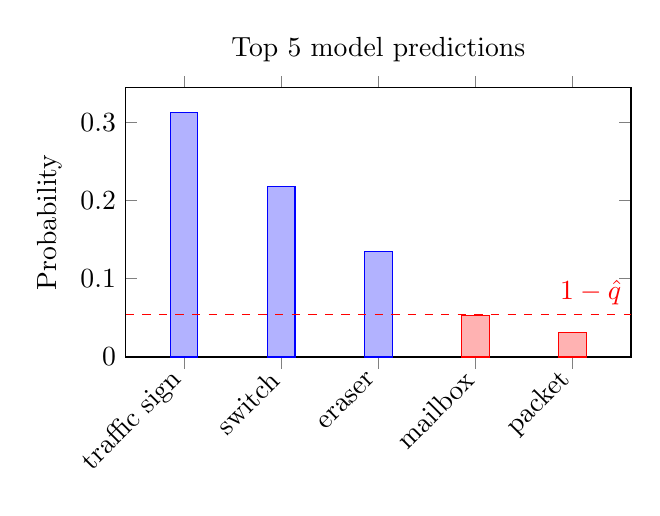
\begin{tikzpicture}
\begin{axis}[
    width=8cm,
    height=5cm,
    title={Top 5 model predictions},
    ybar,
    symbolic x coords={traffic sign, switch, eraser, mailbox, packet},
    xticklabel style={
        rotate=45,
        anchor=east
    },
    ylabel=Probability,
    ymin=0,
    enlarge x limits=0.15,
    bar shift=0pt,
    legend pos=north east,
]

\addplot coordinates {
    (traffic sign, 0.3126)
    (switch, 0.2180)
    (eraser, 0.1347)
    (mailbox, nan)
    (packet, nan)
};

\addplot coordinates {
    (traffic sign, nan)
    (switch, nan)
    (eraser, nan)
    (mailbox, 0.0525)
    (packet, 0.0315)
};

\path (axis cs:{[normalized]1},0.0546) coordinate (aux);
\end{axis}
\draw[red, dashed] (current axis.west|-aux) -- (current axis.east|-aux) node [above left] {\(1 - \hat{q}\)};
\end{tikzpicture}

\end{document}
